\documentclass[11pt]{article}
\usepackage{amsmath,amssymb,amsthm,enumerate,graphicx,hyperref,tikz}
\usetikzlibrary{arrows.meta}

\newtheorem{theorem}{Theorem}
\newtheorem{lemma}[theorem]{Lemma}
\newtheorem{definition}[theorem]{Definition}
\newtheorem{proposition}[theorem]{Proposition}
\newtheorem{corollary}[theorem]{Corollary}
\newtheorem{example}[theorem]{Example}

\title{Intuition Examples for Paper A:\\
2D Grid Surrogates for Free-Face Covering}
\author{Alan J.\ Coppola}
\date{Companion to \emph{Horn Retraction, Roth Extremals, and Espresso-Horn}\\Draft 2026-11-23}

\begin{document}
\maketitle

\begin{abstract}
This companion note collects the Layer~1 geometric sandbox used to develop
intuition for Paper~A: filled/hollow/absent $F/H/.$\ grids, the $2\times 3$ ring
counterexample, the $3\times 3$ face-row vs.\ vertex-row dichotomy,
Link$(\mathrm{opp})$ cost windows, and non-core $P_4$/$P_6$ path sketches.
None of these grid statements is an automatic Layer~0 absolute-minimization theorem;
see the main paper for Horn retraction (H1--H4), Roth extremals, and Espresso-Horn.
\end{abstract}

\section{Scope}
\label{sec:scope}
Paper~A works on Layer~0 cube arrays.  The material below is a
\emph{geometric covering surrogate} (Layer~1): the same reduction code on
vertex-row or face-row tables of F/H/.\ grids yields \emph{grid-surrogate cores},
not Layer~0 cyclic cores, until restated for minterm$\times$cube arrays.

\subsection{Geometric sandbox (Layer~1)}
\label{sec:sandbox}

Filled/hollow/absent grid complexes with \emph{vertex-row} or \emph{face-row}
tables are a \emph{geometric covering surrogate}.  Residuals after the same
reduction code on those tables are \emph{grid-surrogate cores}, not Layer~0
cyclic cores, until the claim is restated for a minterm$\times$cube array.
Theorems~\ref{thm:face-star}--\ref{thm:link-bounds} below are proved and audited
in this sandbox; they are not automatic theorems about absolute cube-array
minimization.

\begin{example}[Suspension sphere]
\label{ex:suspension}
Let $I^k=[0,1]^k$ with its standard cubical decomposition.  Remove the
antipodal vertices $(0,\ldots,0)$ and $(1,\ldots,1)$ together with every cube
containing either vertex, and take face closure.  The result $X_k$ is the
equatorial belt in the suspension $\Sigma S^{k-2}\cong S^{k-1}$: top cells have
cubical dimension $k-2$ and $X_k$ is homotopy equivalent to $S^{k-2}$ ($k=3$
gives a $6$-cycle; $k=4$ a cubical $S^2$).  For $k\ge 3$, $X_k$ is
\emph{not} contractible, and in the geometric construction every top cell is a
prime with no free face.  The code's $k=3$ complex is that 6-cycle and has no
collapsible column.  The code's $k=4$ complex is a shorter stand-in (six
squares) and \emph{does} have free faces, so it is not the negative control
the geometric sentence describes.
\end{example}

\section{Free-face local transform on grids}
\label{sec:main}

\textit{Scope.}  This section is Layer~1 (Section~\ref{sec:sandbox}).  We treat
two row models on F/H/.\ grids.  \emph{Face rows} give a star/essential offset
(Theorem~\ref{thm:face-star}).  \emph{Vertex rows} give the far-side
characterization (Theorem~\ref{thm:far-side}) and the Link$(\mathrm{opp}(f))$
approx window (Theorem~\ref{thm:link-bounds}).  None of these is yet a Layer~0
one-recursion absolute-min theorem for arbitrary arrays of cubes.

\subsection{Absolute theorem (face rows)}
\label{sec:face-star}

\begin{theorem}[Free face $\Rightarrow$ essential star collapse]
\label{thm:face-star}
On a face-row covering table (rows $=$ all proper faces of top cells), if $f$ is
a free face of a top cell~$p$ of unit weight, then $p$ is essential and
\[
\mathrm{opt}(K)=1+\mathrm{opt}(K/p),
\]
where $K/p$ deletes column~$p$ and every row covered by~$p$.  Equivalently, the
geometric star $\mathrm{st}(f)=\{\tau:f\le\tau\}$ witnesses the elementary
collapse that removes~$p$ after paying its weight.
\end{theorem}

\begin{proof}
Freeness among top cells means the face-row for~$f$ is covered only by~$p$, so
$p$ is an essential column.  Essential-column reduction gives the displayed
identity.  (Lean \textsf{theoremA\_essential\_offset}; audited on all free
squares of $2\times2$, $2\times3$, and $3\times3$ grids ---
Table~\ref{tab:star-link}.)
\end{proof}

\subsection{Vertex-row far side and Link$(\mathrm{opp})$ approx}
\label{sec:vertex-link}

Fix a grid-surrogate residual with residual rows~$R\subseteq V(K)$ and
columns~$P$ (unit weights).

\begin{definition}[Far side and transform $T$]
\label{def:far-side}
Let $p\in P$ be a filled square with free face $f$.  The \emph{far side} is
$F_p=(V(p)\cap R)\setminus V(f)$.  The local transform is
$P'=P\setminus\{p\}\cup\{f\}$.  \emph{Decode} swaps a chosen~$f$ back to~$p$;
\emph{put-back} (\textsf{Reduced}) then drops every chosen cube that the rest of
the cover already covers (exact minimum sub-cover for $\le 16$ columns; greedy
beyond).
\end{definition}

\begin{lemma}[Lemma~A]
\label{lem:A}
$\mathrm{opt}(P')\le\mathrm{cost}(C_{\mathrm{out}})$ unconditionally: every
exclude-$p$ cover of~$P$ remains feasible on~$P'$.
\end{lemma}

\begin{lemma}[Lemma~B]
\label{lem:B}
Decode plus put-back returns a feasible cover of~$P$ and never raises cost
(Lean \textsf{lemma\_B\_decode\_putback}).
\end{lemma}

\begin{theorem}[Far-side characterization]
\label{thm:far-side}
With unit weights,
\[
\mathrm{opt}(P')=\mathrm{opt}(P)
\quad\text{if and only if}\quad
\begin{array}{l}
\text{some minimum cover of~$P$ either excludes~$p$,}\\
\text{or covers~$F_p$ using columns other than~$p$.}
\end{array}
\]
\end{theorem}

\begin{proof}
Write $m=\mathrm{opt}(P)$ and $m'=\mathrm{opt}(P')$.
Lemma~\ref{lem:A} gives $m'\le\mathrm{cost}(C_{\mathrm{out}})\le m$, so always $m'\le m$.

($\Leftarrow$) Suppose some minimum cover $S$ of~$P$ excludes~$p$.  Then $S$ is
feasible on~$P'$, so $m'\le|S|=m$, hence $m'=m$.
Suppose instead some minimum cover $S\ni p$ covers $F_p$ by the columns in
$S\setminus\{p\}$.  The near rows $V(f)\cap R$ are covered by~$f$ once $p$ is
replaced by~$f$, and every other residual row of~$S$ is unchanged, so
$(S\setminus\{p\})\cup\{f\}$ is a feasible cover of~$P'$ of cost~$m$.  Thus
$m'\le m$, and with Lemma~\ref{lem:A} we get $m'=m$.

($\Rightarrow$) Suppose $m'=m$, and assume for contradiction that every minimum
cover of~$P$ contains~$p$ and that no such cover covers $F_p$ without~$p$.
Then $\mathrm{cost}(C_{\mathrm{out}})>m$, so every cover of~$P'$ of cost~$m$ must
use~$f$ (otherwise it would be an exclude-$p$ cover of~$P$).  Decoding any such
cover replaces~$f$ by~$p$ and yields a minimum cover of~$P$ that still leaves a
far row uncovered by the complementary columns---contradicting feasibility of the
decoded cover on~$P$, or else forcing an extra column and cost~$>m$.  Hence some
minimum cover excludes~$p$ or covers $F_p$ without~$p$.

Lean records the abstract interface as \textsf{characterization\_iff}; the
Python auditor finds $0$ mismatches on all $32\,288$ vertex-row pairs of
$3\times 3$ grids and on all $1\,013\,750$ pairs of the exhaustive $3\times 4$
audit (\textsf{grid\_collapse\_char\_3x4.json}).
\end{proof}

\begin{proposition}[Row-model dichotomy]
\label{prop:dichotomy}
On the same filled/hollow/absent grids, under \emph{face rows} (all proper faces
as rows) no cyclic core retains a collapsible filled square ($0/4\,149$ cores on
$3\times 3$).  Under vertex rows, $6\,126/9\,770$ cores do.  Thus ``free faces
generalize essential primes'' is the face-row reading; the logic-minimization
problem is the vertex-row reading.
\end{proposition}

\begin{definition}[Link Out-complex]
\label{def:link-out}
Let $f$ be free for square~$p$ and $\mathrm{opp}(f)$ the opposite edge on~$p$.
The vertex-row \emph{Link Out-complex} $\mathrm{Out}_{\mathrm{link}}(p,f)$ has
rows $\bigl(V(\mathrm{lk}(\mathrm{opp}(f)))\cup V(\mathrm{opp}(f))\bigr)\cap R$
and columns all residual top cells meeting those rows except~$p$.  Write
$L=\mathrm{MinCov}(\mathrm{Out}_{\mathrm{link}})$ and
$U=\mathrm{cost}\bigl(\mathrm{Reduced}(M\cup\{p\})\bigr)$ for
$M$ a minimum cover of $\mathrm{Out}_{\mathrm{link}}$.
\end{definition}

\begin{theorem}[Link$(\mathrm{opp})$ cost window]
\label{thm:link-bounds}
For unit-weight vertex-row residuals and free $(p,f)$,
$L\le\mathrm{opt}\le U$.  On all $32\,288$ free pairs of $3\times 3$ grids there
are $0$ violations; the stitch is exact on $96.1\%$ of pairs (gap~$1$ on the
rest).  On the $2\times 3$ ring where the free-face swap fails, $U=\mathrm{opt}$.
\end{theorem}

\begin{proof}[Proof sketch]
Any cover of~$K$ restricts to a cover of the link/collar rows after deleting~$p$,
so $L\le\mathrm{opt}$.  The stitch $\mathrm{Reduced}(M\cup\{p\})$ is feasible, so
$\mathrm{opt}\le U$.  Lean \textsf{theoremC\_window}; Python
\textsf{audit\_link\_bounds}.
\end{proof}

\noindent\textbf{Approx-min certificate.}  Downstream cubical reductions that only
need a cover whose nerve/Stanley--Reisner (or chosen persistence) matches a true
min cover up to a stated checker may use any stitch cover of cost~$\le U$ together
with the window $(L,U)$ as an \emph{admissible approx-min certificate}; optimality
is not claimed unless $U=L$ or an exact oracle agrees.

\begin{example}[Smallest vertex-row sandbox counterexample]
\label{ex:grid2x3}
\textit{Layer~1 only.}  The $2\times 3$ hollow ring with one filled square
(\texttt{H~H / F~H / H~H}) is already free of unique-row essentials on the vertex
table (a grid-surrogate core).  It has $\mathrm{opt}=5$ but $\mathrm{opt}(P')=6$ for
every free face of the square: the far side is uncovered by every minimum cover
without~$p$.  This is \emph{not} yet a Layer~0 counterexample for arrays of cubes
over minterms.  Lean \textsf{grid2x3\_counterexample} checks a $7$-column strip form
by \texttt{decide}/\texttt{native\_decide}.
\end{example}

\begin{figure}[ht]
\centering
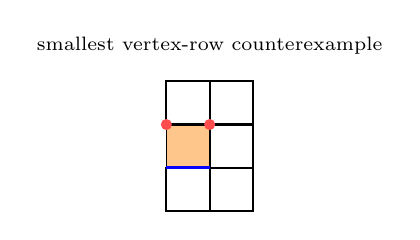
\begin{tikzpicture}[x=0.55cm,y=0.55cm,every node/.style={font=\scriptsize}]
\node[anchor=south] at (1.0,3.4) {smallest vertex-row counterexample};
\draw[fill=white] (0,0) rectangle ++(1,1);
\draw[thick] (0,0) rectangle ++(1,1);
\draw[fill=orange!45] (0,1) rectangle ++(1,1);
\draw[fill=white] (0,2) rectangle ++(1,1);
\draw[thick] (0,2) rectangle ++(1,1);
\draw[fill=white] (1,0) rectangle ++(1,1);
\draw[thick] (1,0) rectangle ++(1,1);
\draw[fill=white] (1,1) rectangle ++(1,1);
\draw[thick] (1,1) rectangle ++(1,1);
\draw[fill=white] (1,2) rectangle ++(1,1);
\draw[thick] (1,2) rectangle ++(1,1);
\draw[blue,very thick] (0,1) -- (1,1);
\fill[red!70] (0,2) circle (2pt);
\fill[red!70] (1,2) circle (2pt);
\end{tikzpicture}
\caption{Smallest vertex-row counterexample shape: filled square~$p$ (orange),
free face~$f$ (blue), far-side vertices (red).  Hollow cells are edge frames.}
\label{fig:grid-cex}
\end{figure}

\begin{definition}[Cover-admissible free face]
\label{def:admissible}
A free face $f\in F(p)$ is \emph{cover-admissible} if every covering-table row
incident to~$f$ is not covered by any original prime $q\neq p$ that fails to
contain~$f$.  This is what the Boolean implementation checks; it is
\emph{not} the far-side condition of Theorem~\ref{thm:far-side}.
\end{definition}

\paragraph{Sufficient condition from the search loop.}
Among checkable predicates on $(p,f)$, the condition
$|F_p|=1$ and $|V(f)\cap R|=1$ fires on $10\,760/32\,288$ ($33.3\%$) of $3\times 3$
vertex-row pairs with \emph{zero} failures, and on a $3\times 4$ sample with zero
failures (\textsf{grid\_collapse\_round2.json}).  The trivial case $F_p=\emptyset$
fires on $17.7\%$ with zero failures and is reported separately.

\subsection{Out\_complex (trimmed) and non-core path witnesses}
\label{sec:outcomplex}

The four-step $\mathrm{Out\_complex}$ procedure (remove $\mathrm{FF}_c$, solve,
return $M$ or $\mathrm{Reduced}(M\cup\{\mathrm{FF}_c\})$) remains a useful Boolean
reformulation: feasibility is unconditional; optimality needs $(H_{\mathrm{out}})$
(Lean \textsf{OutComplex.lean}).  Path witnesses $P_4$/$P_6$ illustrate put-back
and collar lock-in but \emph{are not cyclic cores} (they retain essential edges)
and are not used as core evidence for Theorem~\ref{thm:far-side}.  True cyclic-core
Boolean traps at $n=4$/$n=5$ are recorded in Section~\ref{sec:negative}.

\begin{example}[Coppola--Weiss 2007 cyclic core]
\label{ex:cyccore}
Figure~\ref{fig:cyccore} realizes a nine-cell cyclic core whose graded
covering table is the $9\times 9$ incidence matrix of
Coppola--Weiss~\cite{coppola2007} (Table~1 of the 2006/07 draft).  The six
outer primes $p_1,\ldots,p_6$ each have a free face; the three inner primes
$p_7,p_8,p_9$ do not.  Choosing $p_1$ as the collapsible cell removes that
column, inserts its free-face column(s), and recurses once---after which any
used free face is restored to $p_1$.  The instance is encoded in
\textsf{TopoSpine} as \textsf{coppola\_2007\_graded} (derived typed $T_C$).
\end{example}



\section*{Pointer}
Return to Paper~A for Horn retraction, Espresso-Horn, and Layer~0 cyclic-core
theorems.  Lean checks for grid statements live in \textsf{LocalTransform.lean}
and \textsf{StarLink.lean}.

\end{document}
